\documentclass[conference]{IEEEtran}
\IEEEoverridecommandlockouts
\usepackage{cite}
\usepackage{amsmath,amssymb,amsfonts}
\usepackage{algorithmic}
\usepackage{graphicx}
\usepackage{textcomp}
\usepackage{xcolor}
\usepackage{multirow}
\usepackage{boldline}
\usepackage{stackengine}
\usepackage{siunitx}
\usepackage{floatrow}

\def\BibTeX{{\rm B\kern-.05em{\sc i\kern-.025em b}\kern-.08em
    T\kern-.1667em\lower.7ex\hbox{E}\kern-.125emX}}
\begin{document}

\title{Deep Q-Network \\ Lab 3}


 \author{\IEEEauthorblockN{1\textsuperscript{st} Nicolaas P. Cawood \\ 2376182}
 \and
 {\IEEEauthorblockN{2\textsuperscript{nd} ABC DEF \\ xxxx}}
  \and
 {\IEEEauthorblockN{3\textsuperscript{rd} ABC DEF \\ xxxx}}
   \and
 {\IEEEauthorblockN{4\textsuperscript{th} ABC DEF \\ xxxx}}
}

\maketitle
\section{Introduction}

Atari games have been used to illustrate the potential for reinforcement learning in many studies over the past decade. We implemented the first deep learning model which successfully learned the control policies from only the video feedback of these games instead of memory. The Deep Q-Network \cite{mnih2013playing} and the improved Double Deep Q-Network \cite{van2015deep} were implemented to put test their performances on the classic arcade game of Pong.

\section{The training process}
We followed the training loop illistrated by figure \ref{fig:rl}. The training process was completed in the following order, over 1000000 frame steps
\begin{enumerate}
  \item An $\epsilon$-greedy action is selected, which gives a higher probability of choosing the greedy action as the number of episodes increase.
  \item The action is taken in the environment, and the next state, reward and terminal-condition is observed.
  \item We add the reward to the total rewards for the current episode, and the state, action, reward and next state transition are stored in the experience replay memory.
  \item We use stochastic gradient descent to optimise our policy network weights from a $32$ sample mini-batch from the experience replay memory. The TD loss we optimise are computed as the absolute element-wise error between the policy network and the target network using the Hubert loss, which is less sensitive to outliers than the mean square error.
  \item The target network's weights are updated to the policy network's weights every $1000$ steps.
\end{enumerate}

\begin{figure}[!ht]
    \centering
	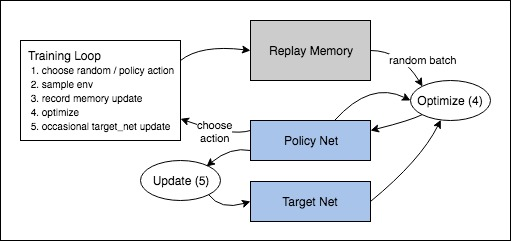
\includegraphics[width=\textwidth]{resources/reinforcement_learning_diagram.jpg}
	\caption{The Deep Q-Network training loop\cite{pytorch}.}
	\label{fig:rl}
	
\end{figure}

\section{Hyperparameters}
We experimented with the "PongNoFrameskip-v4" environment from the OpenAI Gym API. The hyperparameters were captured in appendix \ref{appendix}. We followed the approach used for the training as per the original paper \cite{mnih2013playing}, which include
\begin{itemize}
    \item The rewards were clipped at $1$ and all the negative rewards to $-1$, and
    \item we treated both a win and a loss as the end of an episode.
    \item Mini-batches of size 32 were used as the history of each optimisation step.
    \item An $\epsilon$-greedy behaviour policy was used with $\epsilon$ annealing from $1.0$ to $0.1$ over the first million frames, and fixing it to $0.1$ afterwards, which reduces the exploration of the agent as the training gets closer to the end.
 \end{itemize}   
The RMSProp algorithm was replaced with an Adam optimizer, which is a stochastic gradient decent algorithm and we used the Huber Loss to compute the TD error to minimize.
We also excluded the frame-skipping technique that was used in the original paper. 

\subsection{Q-Network architecture}
We implemented the exact deep neural network architecture from the original paper as described in the Nature DQN version, using the PyTorch API. The model was programmed as a linear stacking of layers, each separated by Rectifier Linear Units (ReLu) and the architecture used followed

\begin{itemize}
    \item The input layer: a convolution layer, with $32$ 8x8 filters and a stride of 4. 
    \item The first hidden layer : a convolution layer, with $64$ 4x4 filters, and a stride of 2. 
    \item The second hidden layer : a convolution layer, with $64$ 3x3 filters, and a stride of 1. 
    \item The third hidden layer : a fully connected linear layer, with an output length of $512$. 
    \item The output layer: a fully-connected linear layer, with a single output for each action.
\end{itemize}  


\bibliographystyle{IEEEtran}
\bibliography{bib}
\clearpage
\appendices
\section{Model hyperparameters}
\label{appendix}
\begin{table}[!ht]
\begin{tabular}{|l|l|l|}
\hline
\textbf{Hyperparameter} & \textbf{Value} & \textbf{Description}                                              \\ \hline
learning rate          & 1e-4 & The rate at which the Q-network parameters are updated using stochastic gradient descent \\
target network update   & 1000           & The number of iterations before each target network update        \\
experience replay size & 1e6  & The memory from which the mini-batches are sampled for the optimisation                  \\
discount factor         & 0.99           & The gamma parameter for the Q-learning update                     \\
intitial exploration    & 1.0            & Initial value for epsilon                                         \\
final exploration       & 0.1            & The final value for epsilon                                       \\
exploration frames      & 1e6            & The number of frames that the epsilon value linearly anneals over \\
no-op max              & 30   & Maximum number of "do-nothing" actions by the agent during the start of an episode       \\
action repeat           & 4              & The number of frames an action is repeated                        \\ \hline
\end{tabular}
\end{table}


\end{document}
